\documentclass[a4paper]{article}
\usepackage[nottoc]{tocbibind}
\usepackage{graphicx}
\usepackage{float}
\graphicspath{ {./images/} }

\begin{document}
\title{Securitatea și confidențialitatea datelor în contextul aplicațiilor mobile}

\author{Ghimpu Lucian Eduard}
\maketitle




\textsc{Conducător științific}

\textsc{Dr. CZIBULA Istvan, Profesor Universitar}

\newpage

\tableofcontents


\section{Introducere}
\subsection{Introducere}
\subsection{Ecosistemul aplicațiilor mobile}
\subsection{GDPR}

\section{Securitatea și confidențialitatea datelor în contextul aplicațiilor mobile}


\subsection{Autentificarea si înregistrarea}
\newpage
\subsubsection{Ceva introducere *}

Indiferent ca vorbim de aplicatii web, desktop sau mobile, majoritatea folosesc 
o metoda de autentificare. Auntentificarea șî înregistrarea stau la baza
problematicii securitatii datelor. In clasamentul OWASP Top 10 din 2017 \cite{owasp-top10-2017}, 
problemele legate de autentificare si gestiunea sesiunii, sunt clasate pe locul 2. Iar in
clasamentul OWASP top 10 Mobile din 2016 \cite{owasp-top10-mobile}, autentificare nesigura
si autorizarea necurespunzatoare sunt clasate pe locul 4, respectiv 6.

Unicitatea aplicatilor mobile este data de faptul ca un dispozitiv mobil
poate devenii accesibil oricarui persoane datorita portabilitatii lor. Un dispozitiv mobil
poate fi furat, pierdut sau accesat temporal de o persoana necunoscuta fara permisiunea
posesorului. Prin urmare nevoia de un sistem de autentificare robust este mandatorie 
atunci cand vorbim de aplicatii care gestioneaza date sensibile (aplicatii financiare, sociale,
medicale, etc...).

\bigskip

In cadrul aplicatiilor mobile, autentificarea se poate face prin mai multe metode. De la
simpla autentificare prin utilizator si parola, pana la utilizarea de sezori biometrici.
Mitigari clasice precum impunerea unei parole sigure raman valabile si in 
contextul aplicatiilor mobile.


Pentru alegerea metodei de autentificare trebuie sa ne punem in prima instanta urmatoarele doua
intrebari:

\begin{itemize}
    \item Care este scopul aplicatiei? O aplicatie care notifica utilizatorul despre starea meteo poate 
    ca nu ar avea nevoie de autentificare prin senzori biometrici. 
    \item Aplicatia gestioneaza date confidentiale? Un exemplu potrivit ar fi o aplicatie precum BT pay, care gestioneaza 
    contul curent al unui utilizatorul
    se foloseste de mai multe metode de autentificare, o data prin datele de logare, iar apoi
    prin senzori biometrici.
\end{itemize}

Dupa ce ne este clar care este scopul aplicatiei si cu ce fel de date lucreaza, 
putem include una sau mai multe metode de autentificare bazate dupa urmatorii
factori:

\begin{enumerate}
    \item Ceva ce utilizatorul stie (parola, pin etc\dots)
    \item Ceva ce il defineste pe utilizator (amprenta, retina)
    \item Ceva ce utilizatorul detine (parole generate temporal)
\end{enumerate}

\begin{figure}[H]
\centering
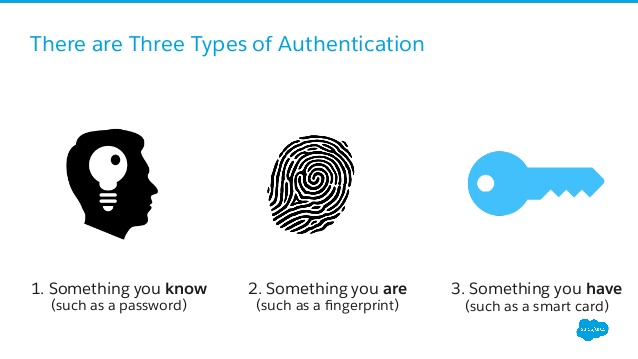
\includegraphics[height=4cm]{3ways.jpg}
\caption{Metode de autentificare \cite{3ways-auth}}
\end{figure}

\subsubsection{JWT si OAuth2}

Majoritatea aplicatiilor de azi se folosesc de cea mai simpla forma de autentificare,
prin folosirea de credentiale (ceva ce utilizatorul stie) si unui token de acces (ceva
ce utilizatorul detine). Utilizatorul isi creeza cont pentru o anumita aplicatie, foloseste
credentialele pentru a se loga, cererea de autentificare ajunge la server unde se verifica
credentialele iar apoi se genereaza un token care va fi folosit de utilizator pentru a accesa
diferite resurse in aplicatie.

Scenariu descris anterior se refera la folosirea de JWT (JSON Web Token), un standard (RFC 7519) \cite{rfc-7519} 
adoptat de multe aplicatii mobile in zilele noastre. 
JSON Web Token este o metoda sigura de autorizare a trasferului
de informatii intre doua parti \cite{jwt}, deobicei 
clientul mobil si serverul la care se face cererea. Clientul revendica de la server
o dovada, un token, care apoi este folosit de client pentru a accesa diferite 
resurse.

Din punct de vedere tehnic, un JWT are urmatoarea forma 11111.22222.33333 si este
alcauit din 3 parti:

\begin{enumerate}
    \item Antetul (Header)
    \item Datele utile (Payload)
    \item Semnatura (Signature)
\end{enumerate}


\begin{figure}[H]
    \begin{minipage}[c]{0.67\textwidth}
        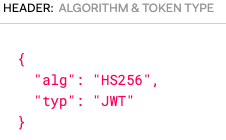
\includegraphics[width=\textwidth]{jwt-header.png}
    \end{minipage}\hfill
    \begin{minipage}[c]{0.3\textwidth}
        \caption{Antetul unui JWT, alcatuit din tipul de algoritm 
        de inregistrare (HS256) si tipul de token (JWT).}
    \end{minipage}
\end{figure}

\begin{figure}[H]
    \begin{minipage}[c]{0.67\textwidth}
        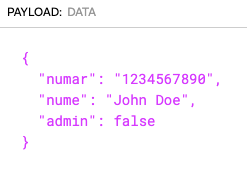
\includegraphics[width=\textwidth]{jwt-payload.png}
    \end{minipage}\hfill
    \begin{minipage}[c]{0.3\textwidth}
        \caption{Partea utila al unui JWT contine date sau permisiuni
        pe care clientul le are.}
    \end{minipage}
\end{figure}

\begin{figure}[H]
    \begin{minipage}[c]{0.67\textwidth}
        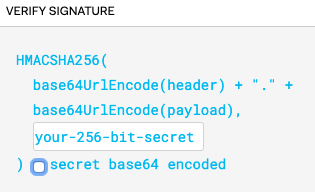
\includegraphics[width=\textwidth]{jwt-sign.png}
    \end{minipage}\hfill
    \begin{minipage}[c]{0.3\textwidth}
        \caption{Semnatura unui JWT este alcatuita din antetul encodat, 
        datele encodate, algoritmul folosit in antet si un secret. Semnatura are rolul
        de a oferi o metoda de verificare pentru a asigura ca continutul nu a fost 
        modificat }
    \end{minipage}
\end{figure}

\begin{figure}[H]
    \begin{minipage}[c]{0.67\textwidth}
        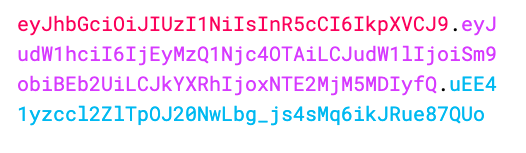
\includegraphics[width=\textwidth]{jwt-all.png}
    \end{minipage}\hfill
    \begin{minipage}[c]{0.3\textwidth}
        \caption{
            JWT va fi format in final 
            de 3 siruri de caractere de tip Base64-URL separate prin punct. }
    \end{minipage}
\end{figure}


O data ce clientul detine un token, acesta trebuie tratat cu multa grija 
in cadrul unei aplicatii. Acesta poate fi folosit mai apoi in antetul tuturor 
cererilor de tip HTTP sub forma Authorization: Bearer <token>. Din acest motiv 
cel mai probabil se doreste salvarea token-ului in memoria locala a dispozitivului
mobil pentru a putea fi apoi folosit in viitor. Acesta poate fi criptat iar la randul 
lui la nivelul clientului, desi in mod nativ atat pe android cat si pe ios exista metode
sigura de stocare a date de tip token (SharedPreferences in mod private pe Android si
keychain pe iOS).

Pentru un nivel si mai mare de siguranta, se poate limita durata de timp
pe care este valabil un token. Spre exemplu aplicatia BT Pay foloseste un token
care este valid tip de 10-15 minute. Dupa ce token-ul expira, utilizatorul este nevoit
sa se autentifice din nou.

Avantajul principal pe care il ofera JWT este facilitatea prin care se demareaza tot procesul
prin care un client isi revendica datele sau drepturile de la un server. 
Un alt aspect important il reprezinta faptul ca in spate, totul se produce folosit obiecte
de tipul JSON, obiecte care sunt extrem de raspandite in orice limbaj de programare
si in tot internetul.

\subsubsection{Autentificare prin senzori biometrici}
\subsubsection{Autentificare prin factori multiplii}

\subsection{Comunicarea cu serverul si servicii (networking) *}
\subsubsection{HTTP și HTTPS}
\subsubsection{Alte canale de comunicare (SMS)}
\subsubsection{Web sockets}

\subsection{Persistența datelor}
\subsubsection{Metode de persistare a datelor}
\subsubsection{Criptografie}
\subsubsection{Gestionarea datelor sensibile}

\subsection{Alți factori}
\subsubsection{Permisiuni}
\subsubsection{Webviews}
\subsubsection{Distribuirea aplicației}
\subsubsection{Probleme specifice pe anumite platforme}


\section{Medicarium}
\subsection{Analiza aplicației}
\subsubsection{Problematica}
\subsubsection{Cazuri de utilizare}

\subsection{Proiectarea aplicației}
\subsubsection{Arhitectura}
\subsubsection{UML ceva???}

\subsection{Implementarea aplicației - Serverul și serviciile}

\subsubsection{Server REST}
\subsubsection{Node.js}
\subsubsection{MongoDB}
\subsubsection{Rute disponibile}
\subsubsection{Autentificare in doi pași}

\subsection{Implementarea aplicației - Clientul mobil}
\subsubsection{Android Jetpack}
\subsubsection{Kotlin}
\subsubsection{Autentificarea}
\subsubsection{Securitatea aplicației}
\subsubsection{Gestionarea permisiunilor}
\subsubsection{Gestionarea fisierelor}

\subsection{Testarea}

\section{Manual de utilizare}

\section{Concluzii}




\newpage

\listoffigures

\begin{thebibliography}{9}

    \bibitem{owasp-top10-2017}
    OWASP Top 10 2017
    \\\texttt{https://www.owasp.org/images/7/72/OWASP\_Top\_10-2017\_\%28en\%29.pdf.pdf}

    \bibitem{owasp-top10-mobile}
    OWASP Top 10 Mobile 2016 
    \\\texttt{https://www.owasp.org/index.php/Mobile\_Top\_10\_2016-Top\_10}

    \bibitem{3ways-auth}
    3 types of Authentication
    \\\texttt{https://www.slideshare.net/awesomeadmin/secure-your-salesforce-org-with-twofactor-authentication}
    
    \bibitem{rfc-7519}
    RFC 7519 JWT
    \\\texttt{https://tools.ietf.org/html/rfc7519}

    \bibitem{jwt}
    JSON Web Token (JWT)
    \\\texttt{https://tools.ietf.org/html/rfc7519}

    \bibitem{enisa-2019}
    ENISA,
    Privacy and data protection in mobile applications, 29.01.2019
    \\\texttt{https://www.enisa.europa.eu/publications/privacy-and-data-protection-in-mobile-applications}

    \bibitem{enisa-2017}
    ENISA,
    Smartphone Secure Development Guidelines, 27.02.2017,
    \\\texttt{https://www.enisa.europa.eu/publications/smartphone-secure-development-guidelines-2016}

    \bibitem{enisa-2017}
    OWASP Mobile Application Security Verification Standard,
    \\\texttt{https://github.com/OWASP/owasp-masvs}


\end{thebibliography}   

\end{document}